%DO NOT MESS AROUND WITH THE CODE ON THIS PAGE UNLESS YOU %REALLY KNOW WHAT YOU ARE DOING
\chapter*{Theory} 
\addcontentsline{toc}{chapter}{Theory}

\section{ Image Source Approach } \label{ Image Source Approach }
\noindent The wave field within a homogeneous waveguide can be interpreted as the superposition of infinitely many spherical waves that are reflected at the boundaries.
\begin{figure}[H]
\centering
{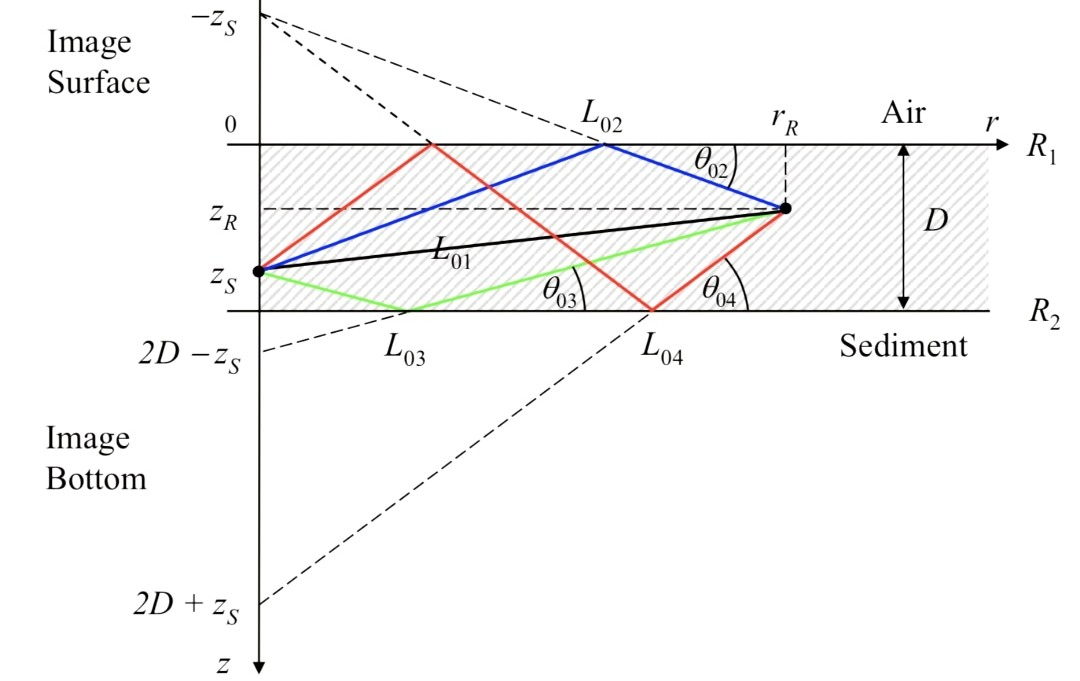
\includegraphics[scale=0.35]{usp1.jpg}}
\caption{ Image source technique }
\end{figure}
\noindent  As a first approximation, the sound pressure in the waveguide can be determined by superimposing the four contributions indicated in the Figure 1, i.e.
\begin{equation}
\textit{$P(r_R, z_R,\omega)$} = A(\omega) \Bigg( \frac{e^{-jkL_{01}}}{L_{01}} + R_{1}(\theta_{02},\omega) \frac{e^{-jkL_{02}}}{L_{02}} +  R_{3}(\theta_{03},\omega) \frac{e^{-jkL_{03}}}{L_{03}} +  R_{4}(\theta_{04},\omega) \frac{e^{-jkL_{04}}}{L_{04}}  \Bigg)
\end{equation}
\noindent with
\begin{equation}
\begin{gathered} 
L_{01}  = \sqrt{r_{R}^{2} + ( z_{R} - z_{S})^{2}} \\
L_{02}  = \sqrt{r_{R}^{2} + ( z_{R} + z_{S})^{2}} \\
L_{03}  = \sqrt{r_{R}^{2} + (2D - z_{S} - z_{R})^{2}} \\
L_{04}  = \sqrt{r_{R}^{2} + (2D + z_{S} - z_{R})^{2}}
\end{gathered} 
\end{equation}
\noindent and
\begin{equation}
\begin{gathered} 
\theta_{02}  = arctan((z_{S} + z_{R}) / r_{R}) \\
\theta_{03}  = arctan((2D - z_{S} - z_{R}) / r_{R}) \\
\theta_{04}  = arctan((2D + z_{S} - z_{R}) / r_{R})
\end{gathered} 
\end{equation}
\noindent Continuation of the image source technique in multiples m = 1,2,... of groups of four contributions provides
\begin{equation}
\begin{gathered} 
\textit{$P(r_R, z_R,\omega)$} = A(\omega)\sum_{m=0}^{\infty} \Bigg( R_{1}^{m}(\theta_{m1},\omega)  R_{2}^{m}(\theta_{m1},\omega)  \frac{e^{-jkL_{m1}}}{L_{m1}} + \\
 + R_{1}^{m+1}(\theta_{m2},\omega)  R_{2}^{m}(\theta_{m2},\omega)  \frac{e^{-jkL_{m2}}}{L_{m2}} +  R_{1}^{m}(\theta_{m3},\omega)  R_{2}^{m+1}(\theta_{m3},\omega)  \frac{e^{-jkL_{m3}}}{L_{m3}} + \\
 +  R_{1}^{m+1}(\theta_{m4},\omega)  R_{2}^{m+1}(\theta_{m4},\omega)  \frac{e^{-jkL_{m4}}}{L_{m4}} \Bigg)
\end{gathered}
\end{equation}
\noindent with
\begin{equation}
\begin{gathered} 
L_{m1}  = \sqrt{r_{R}^{2} + (2Dm - z_{S} + z_{R})^{2}} \\
L_{m2}  = \sqrt{r_{R}^{2} + (2Dm + z_{S} + z_{R})^{2}} \\
L_{m3}  = \sqrt{r_{R}^{2} + (2D(m+1) - z_{S} + z_{R})^{2}} \\
L_{m4}  = \sqrt{r_{R}^{2} + (2D(m+1) + z_{S} + z_{R})^{2}}
\end{gathered} 
\end{equation}
\noindent and
\begin{equation}
\begin{gathered} 
\theta_{m1}  = arctan \Big((2Dm - z_{S} + z_{R}) / r_{R} \Big) \\
\theta_{m2}  = arctan \Big((2Dm + z_{S} + z_{R}) / r_{R} \Big) \\
\theta_{m3}  = arctan \Big((2D(m+1 ) - z_{S} - z_{R}) / r_{R} \Big) \\
\theta_{m4}  = arctan \Big((2D(m+1 ) +  z_{S} - z_{R}) / r_{R} \Big)
\end{gathered} 
\end{equation}
\noindent Taking into account that the reflection coefficients at the ocean surface and bottom can be approximated by \\
\makebox[\textwidth]{ $\textit{R} \approx -1, water-air-interface $}
\makebox[\textwidth]{ $\textit{R} \approx 1, water-hard bottom-interface $}
\noindent the calculation of the sound pressure simplifies to
\begin{equation}
\textit{$P(r_R, z_R,\omega)$} = A(\omega)\sum_{m=0}^{\infty} \Bigg(  \frac{e^{-jkL_{m1}}}{L_{m1}} -
\frac{e^{-jkL_{m2}}}{L_{m2}} +  \frac{e^{-jkL_{m3}}}{L_{m3}} - \frac{e^{-jkL_{m4}}}{L_{m4}} \Bigg)
\end{equation}
